\chapter{Implementation}

\section{System Architecture}
The design rules for each joint are held as data files rather than as code. Each file records the empirical proportions of the joint, the source of each proportion, the default allowable stresses and the preferred size series. The calculation code reads these files. Two consequences follow. The source of any dimension can be reported to the user at the moment it is computed, and a correction to a proportion is a change to data rather than to code.

\section{Software Tools}
Table~\ref{tab:tools-sw} lists the tools used. All of them other than the language model are open source.

\begin{table}[h]
\centering
\caption{Software tools used in the implementation}
\label{tab:tools-sw}
\begin{tabularx}{\textwidth}{llX}
\toprule
Function & Tool & Remark \\
\midrule
Solid modelling & CadQuery 2.8 on the OCCT kernel & open source, scripted parametric modelling \\
Drawing sheet and DXF & FreeCAD, headless & projection, dimensioning and title block \\
Finite element analysis & CalculiX with gmsh & linear static, single component \\
Interpretation of the requirement & Claude language model & parameter extraction only \\
Application & Python standard library server & no external web framework \\
Deployment & container on Vercel & no installation required of the user \\
\bottomrule
\end{tabularx}
\end{table}

\section{Implementation of the Joints}
Each joint is implemented as a module exposing the same interface: a sizing function, a list of failure checks, a geometry builder and a set of dimension specifications for the drawing sheet. Adding a joint therefore requires no change to the surrounding system, which allowed the gib and cotter joint to be added after the other five were complete.

The gib and cotter joint requires particular comment. Unwin gives the division of the breadth and the thickness of the gib and cotter but gives no proportions for the strap. Rather than adopt a ratio from an unrelated source or invent one, every dimension the source does not supply is sized against a failure check until that check is satisfied. No dimension of that joint is therefore unsupported: each is either taken from the source or derived from a stated failure mode.

\section{User Interface}
The system is used through a web browser and is arranged as three panels, as shown in Figure~\ref{fig:landing}. The left panel holds the requirement, the duty sliders, the material selection and the follow-up questions. Moving a slider re-sizes the joint and repeats the checks live. The material selection reports the mass and cost of the design, and the user may add materials of their own. The centre panel shows the three-dimensional model in four views: assembled, exploded, section, and a view colouring the weak spots by utilisation. The right panel carries five tabs: Checks, Dimensions, Drawing, Files and Working, the last of which prints the complete calculation with every value substituted. Light and dark themes are provided.

Five textbook cases can be run with one click: Bhandari Example 4.5, Problem 4.1, NPTEL Question 2, Bhandari Example 4.2 (cotter joint) and the default case. Each displays a table comparing the answer printed in the book with the answer produced by the software.

\begin{figure}[h]\centering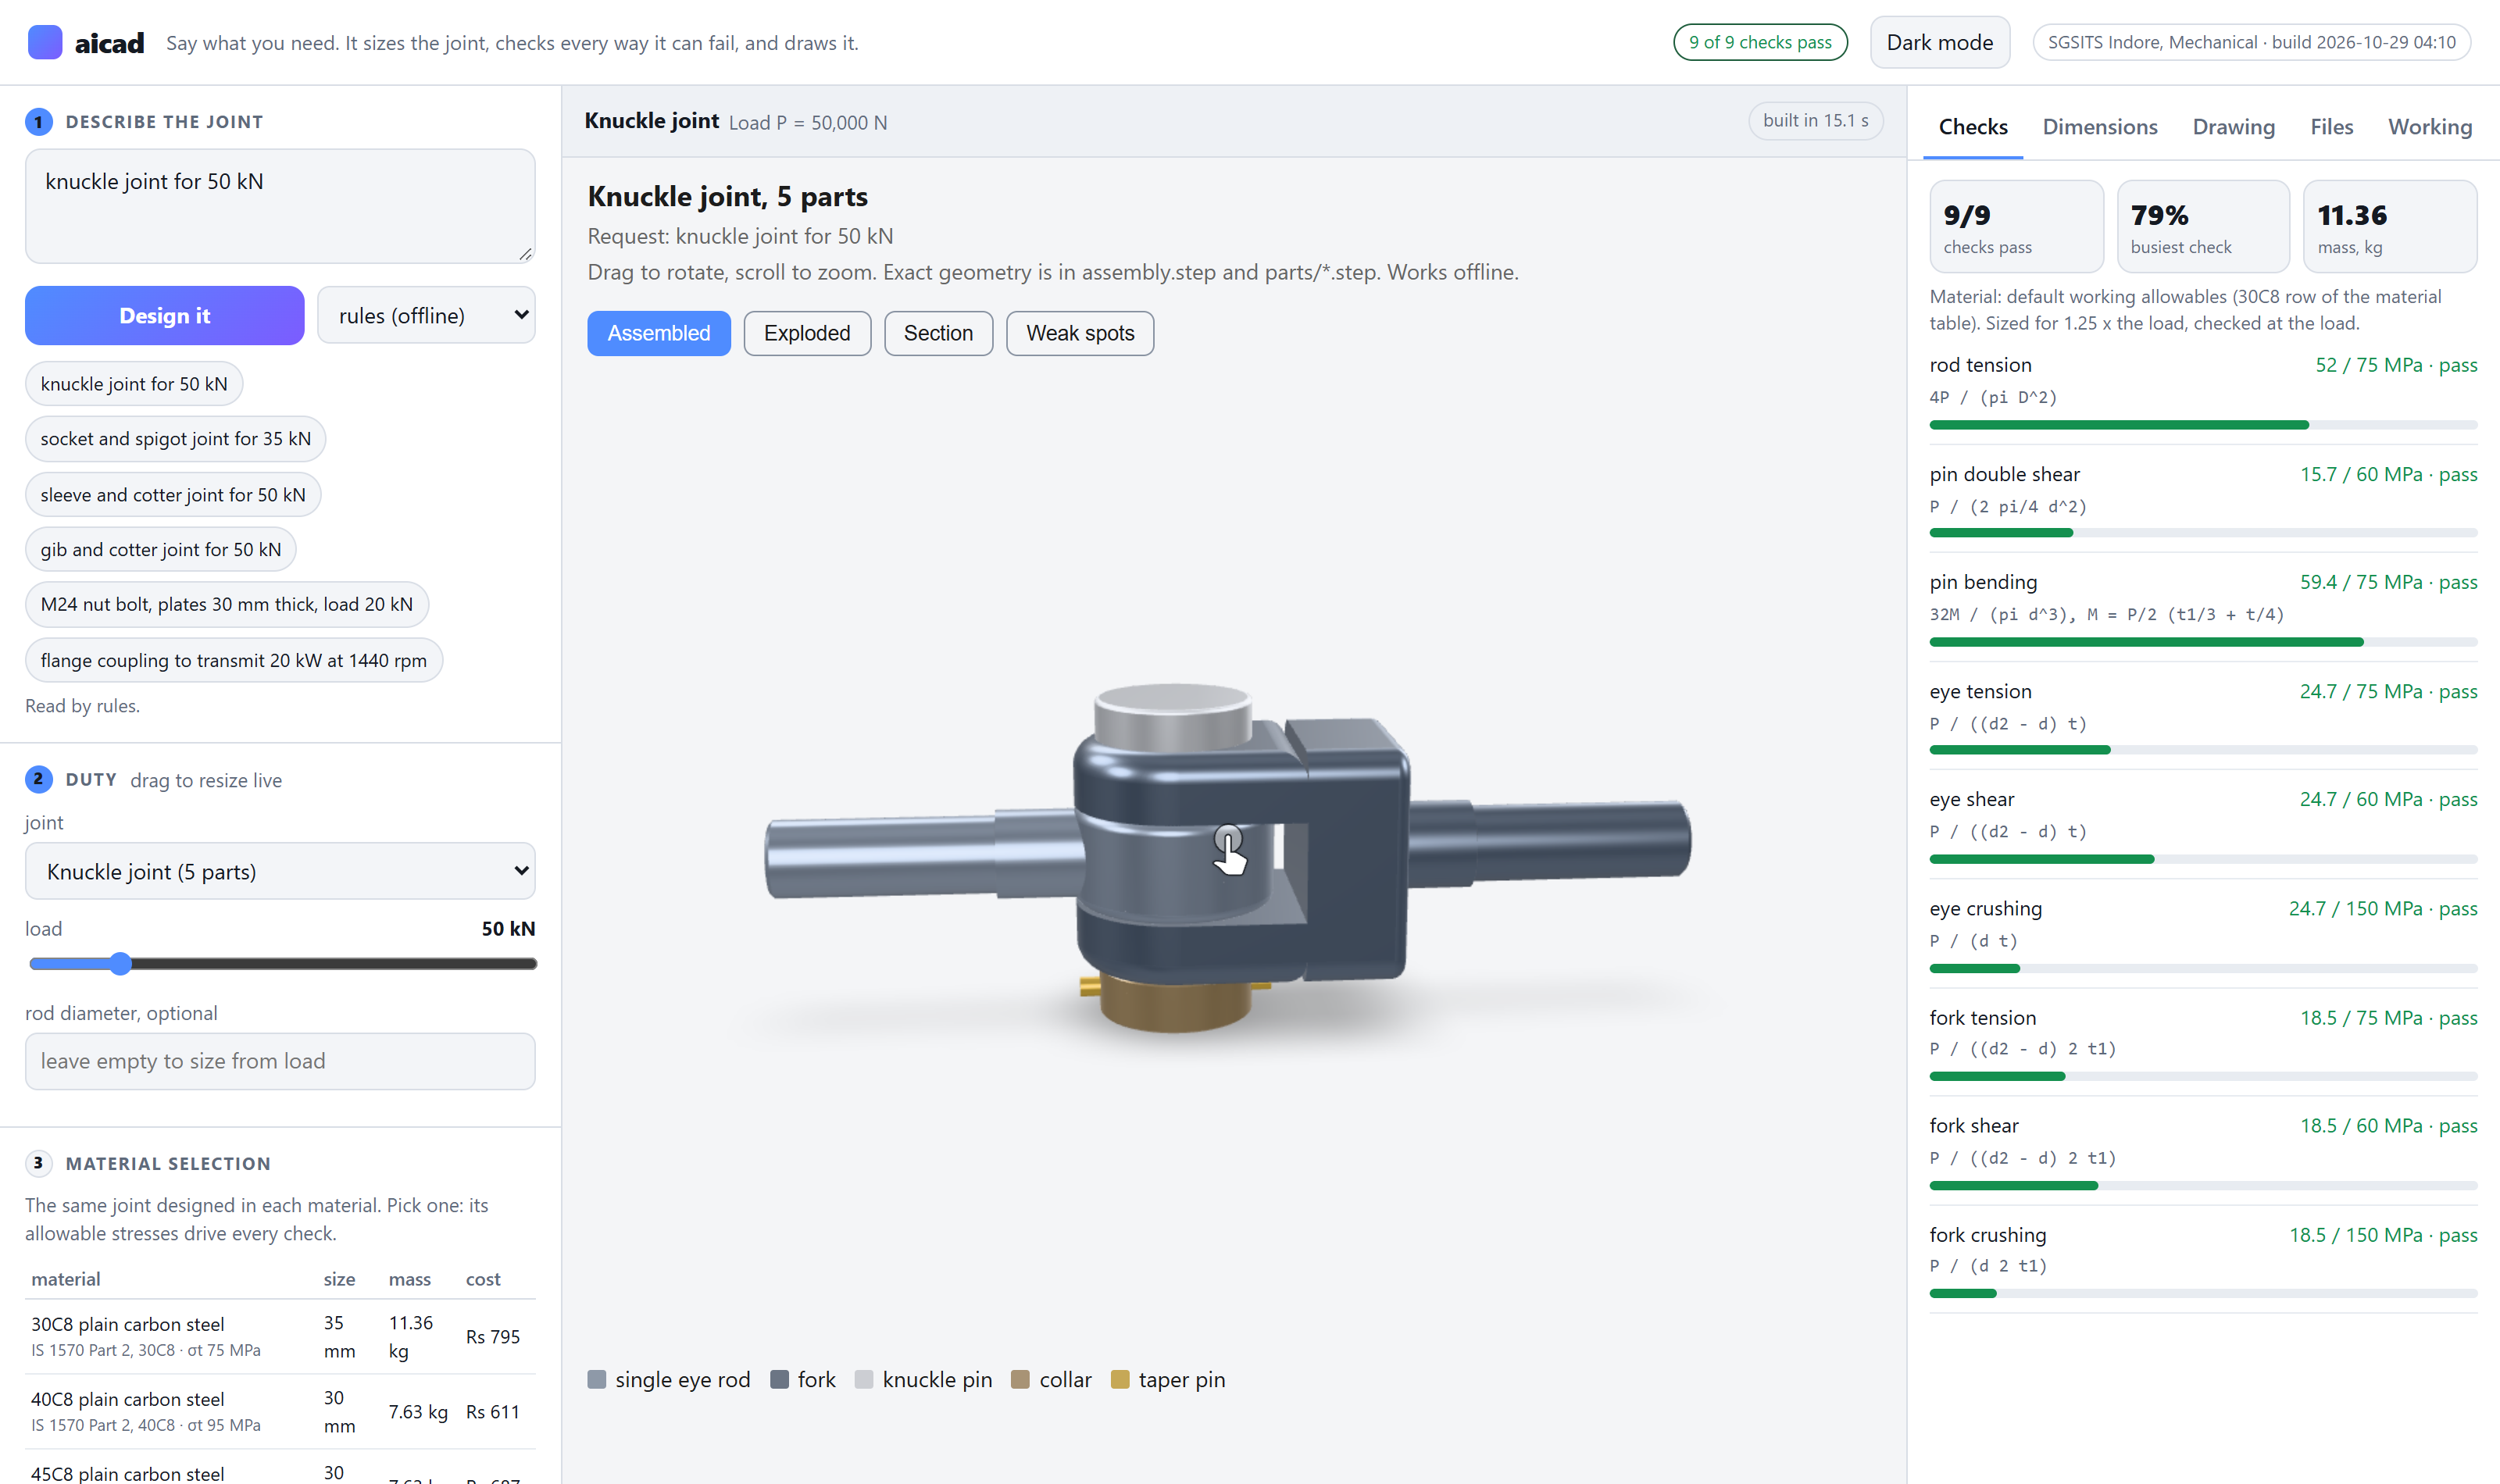
\includegraphics[width=\textwidth,keepaspectratio]{fig/landing.png}\caption{The web application after a design: requirement and sliders, material selection, 3D model, and failure checks}\label{fig:landing}\end{figure}

\section{Build Time}
The time taken by each stage of a build was measured. Sizing and the nine failure checks take under 1 ms, and the solid models take about 0.9 s. The drawing sheet produced by FreeCAD accounts for about 33 s of the 35 s build. Three changes follow from this measurement. The model and the failure checks are now returned first, in about 2 to 5 s, while the drawing sheet is produced in the background, so that the user can read the result while the sheet is being drawn. Results are cached per input, so that a repeated request does not repeat the work. The five textbook cases are built in advance.

\section{Verification of the Implementation}
The implementation is covered by 301 automated tests, which are executed on every change. They cover the sizing arithmetic, the generated geometry, the interpretation of requirements, the drawing sheet, the web interface and the finite element facility. Among them are tests which assert the results printed in the textbook problems, and tests which assert that the source discrepancies recorded in Chapter~7 are genuine, so that the system cannot subsequently be altered to reproduce the printed answers without a test failing.

One class of test detected an error that no dimensional check could have detected. The geometry tests compare the solids of every pair of components and require that no two occupy the same space. That test found a hooked gib modelled 1.25 mm inside the strap, an error invisible in the dimension list because every individual dimension was correct.
